
%%%%%%%%%%%%%%%%%%%%%%%%%%%%%%%%%%%%%%%%%%%%%%%%%%%%%%%%%%%%%%%%%%%%%%%%%%%%%%%%
%%%%%%%%%%%%%%%%%%%%%%%%%%%%%%%%%%%%%%%%%%%%%%%%%%%%%%%%%%%%%%%%%%%%%%%%%%%%%%%%

\section{Mickey mousing}
\label{sec:mikeymousing}
\index{Musicalidade!Mickey mousing}
%onomatopeia andante


\subsection{Mickey mousing no cinema}

``Mickey mousing'' refere-se à técnica empregada nos primeiros filmes de desenhos animados produzidos por Walt Disney,
onde era evidente que a música reforçava, e estava sincronizada, 
com a ação vista na cena \cite{butterworth2011dance} \cite[pp. 62]{kalinak2010film}.
A técnica foi vista por primeira vez no filme ``Steamboat Willie'' (1928),
sendo este o primeiro filme que Walt Disney fez sobre ``Mickey mouse'' \cite[pp. 37]{wegele2014max}.

O termo ``mickey mousing'' é usado no cinema para indicar a sincronização da música com os movimentos em cena,
geralmente com o objetivo de enfatizar a ação narrativa por meio desta coordenação de música e imagem
  \cite{butterworth2011dance} \cite[pp. 62]{kalinak2010film}.


\begin{example}
Quando um personagem na cena desce abruptamente ou cai, 
se executa  de forma sincronizada na música um metáfora da queda,
como uma dissonância ou um aumento abrupto dos tons das notas musicais.
\end{example}

Atualmente a música cinematográfica não usa cotidianamente ``mickey mousing'' como recurso,
e sim técnicas como o ``\hyperref[ref:Underscoring]{\textbf{underscoring}}''\footnote{
A técnica do ``underscoring'' e descrita na Pag. \pageref{ref:Underscoring}.} e 
o ``\hyperref[subsec:LeitmotivCine]{\textbf{leitmotif}}''\footnote{
A técnica do ``leitmotif'' e descrita na Pag. \pageref{subsec:LeitmotivCine}.} \cite[pp. 37]{wegele2014max}.
Isto é devido a que o ``mickey mousing'' é considerado por alguns cineastas como simplista ou vulgar,
este é o caso do cineasta Jean Cocteau, que em 1954 chamou a técnica como: ``A mais vulgar de todas as técnicas de música cinematográfica'' \cite[pp. 37]{wegele2014max}.
Porem a técnica como toda ferramenta, é tão boa quanto o uso que se lhe da;
assim, podemos ver o caso do compositor do cinema americano Max Steiner,
que usou a técnica do ``mickey mousing'' em dois momentos importantes do filme ``Casablanca'' (1942);
primeiro quando Ingrid Bergman aponta com um arma a Henry Bogart para forçá-lo a dar-lhe o visto de saída,
e na segunda vez quando o capitão Renault joga fora uma garrafa de 
``Vichy water''\footnote{Água mineral natural das nascentes da cidade francesa de Vichy.} na lixeira;
esta última ação marcava simbolicamente o fim de sua colaboração com o regime \cite[pp. 38]{wegele2014max}.



\subsection{Mickey mousing na dança} 

O ``Mickey mousing'' consiste em realizar nossos movimento de dança,
seguindo a música, nota por nota, frase a frase, e dinâmica a dinâmica,
atrelando de forma temporal a música com nossa dança
\cite[pp. 460]{preston1995dance}.

Geralmente o termo ``mickey mousing'' é usado para descrever 
uma dança que imita à música de forma literal e sincronizada, causando um efeito humorístico;
o termo também pode ser usado de forma pejorativa, 
para indicar que um dançarino depende muito dos padrões rítmicos da música \cite{butterworth2011dance}.
Existe um grande consenso entre os profissionais da dança do século 20,
que a dança não deveria seguir literalmente à música, com relações de um-a-um, 
pois esta tende a virar simples ou infantil \cite[pp. 242-243]{dithmer2002another}.

Constant Lambert,  compositor e maestro, condutor do ballet britânico,
indicava que traduções literais de uma linguagem a outra são sempre insatisfatórias 
e usualmente ridículas \cite[pp. 242-243]{dithmer2002another}.
Na mesma linha de pensamento, o compositor Norman Lloyd,
indica que seguir literalmente à musica provoca um efeito de desenho animado,
conhecido no âmbito fílmico como ``mickey mousing''
\cite[pp. 242-243]{dithmer2002another}.

\subsubsection{Visualização musical na dança}
\label{subsubsec:musicvisualization}
\index{Musicalidade!Visualização musical}
Este termo foi cunhado por ``Ruth St. Denis'' (1877-1968) 
para descreve os solos de dança improvisação  de ``Isadora Duncan'' (1878-1927),
usando músicas de Chopin, Gluck e Beethoven \cite{butterworth2011dance} \cite[pp. 473]{runco1999encyclopedia}.
Na sua interpretação, 
Isadora Duncan mostrava mediante sua dança as emoções que eram evocadas nela pela música 
ou aspectos dela, procurando dar uma representação visual à musica
\cite{butterworth2011dance} \cite[pp. 473]{runco1999encyclopedia};
assim, na visualização musical a dança procura descrever as dinâmicas, a rítmica, o fraseio 
e outros aspectos da música \cite[pp. 29]{schrader2005sense}.

A differencia de Isadora Duncan que explorava a a componente emocional da música na sua representação visual,
Ruth St. Denis inventou uma serie de coreografias que davam equivalencia a estruturas musicais,
como harmonia, melodia \cite[pp. 149]{walden2013representation} seguindo uma linea mais literal,
e apegada a pauta musical.

Mesmo que em alguns casos se relacione à visualização musical com o ``mickey mousing'',
existe uma sutil diferencia; quando aplicamos ``mickey mousing'' na dança, 
realizamos uma  tradução literal da pauta aplicando simplesmente um conjunto de regras (tabela de mapeamento),
já na visualização musical existe um esforço imaginativo entre a pauta e cada movimento na dança \cite[pp. 177]{acocella2004mark},
Entre o ``mickey mousing'' e a visualização musical existe a mesma diferencia que entre,
um software de tradução (tradução literal) e uma pessoa fazendo de interprete e guia.
Uma representação gráfica destes conceitos pode ser vista na Figura \ref{fig:musicvisualization}.

\begin{figure}[h!]
    \centering
    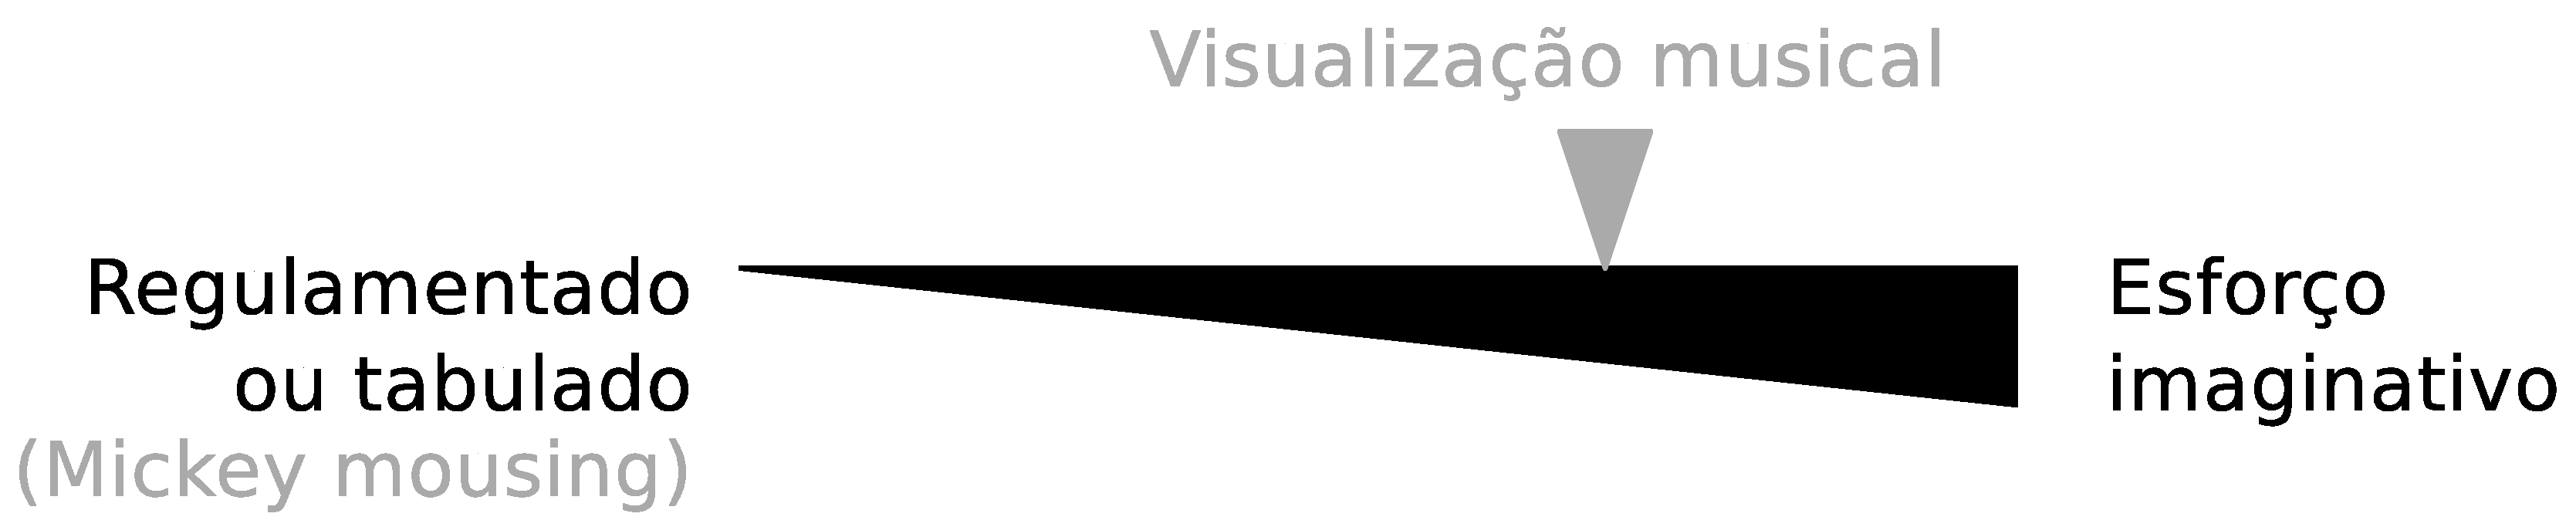
\includegraphics[width=0.9\textwidth]{chapters/cap-musicalidade-tecnica/musicvisualization.eps}
    \caption{Visualização musical na dança.}
    \label{fig:musicvisualization}
\end{figure}

\subsection{Treinando Mickey mousing na dança} 
Nossos treinamentos, usando a técnica de ``mickey mousing'',
seguirão os conceitos já explicados nas seções anteriores;
de modo que em nossos movimentos exista uma relação de sincronia e
literalidade com a musica que usemos.
É claro que ao principio é difícil imaginar-nos como conseguir isto;
porem, um interessante método para inciar este treinamento, 
seria dividir nosso corpo em diferentes instrumentos musicais, 
e atribuir estes um sonido ou motivo na musica tenhamos escolhido.

As partes de nosso corpo que poderíamos usar são:
\begin{itemize}
\item A cabeça, realizando balanços ou simplesmente girar ela para olhar a algum lado.
\item Os ombros, com balanços no \hyperref[def:PlanoFrontal]{\textbf{plano frontal}} ou 
no \hyperref[def:PlanoAxial]{\textbf{plano axial}}.
\item O quadril, com movimentos circulares no plano axial, ou balanços no plano frontal.
\item Os pés, pisando em cada nota musical.
\end{itemize}
Ou também poderíamos usar alguma combinação de movimentos,
o limite esta na nossa imaginação.
Podemos ver propostas de treinamento de ``mickey mousing'' nos Exemplos \ref{ex:mickeymousing-1} e \ref{ex:mickeymousing-2}.

\begin{example}[Dividindo o corpo em dois instrumentos musicais:]
\label{ex:mickeymousing-1}
Neste exercício para treinar a técnica ``mickey mousing'', 
usaremos nossos pés e nosso ombros como dois instrumentos separados,
acompanhando em todo momento a frase musical mostrada na Figura \ref{fig:mickey-mousing-1-1},
\begin{itemize}
\item Nossos pés acompanharão cada figura musical executada pela clave, 
fazendo uma pisada por vez.
\item Nossos ombros (ou o torax) farão um movimento rápido acompanhando o triangulo;
este movimento é feito a escolha nossa, 
e pode ser feito no \hyperref[def:PlanoFrontal]{\textbf{plano frontal}} (comum em samba) ou 
no plano \hyperref[def:PlanoAxial]{\textbf{plano axial}} (comum em salsa).
\end{itemize}
\end{example}
\begin{figure}[h!]
    \centering
    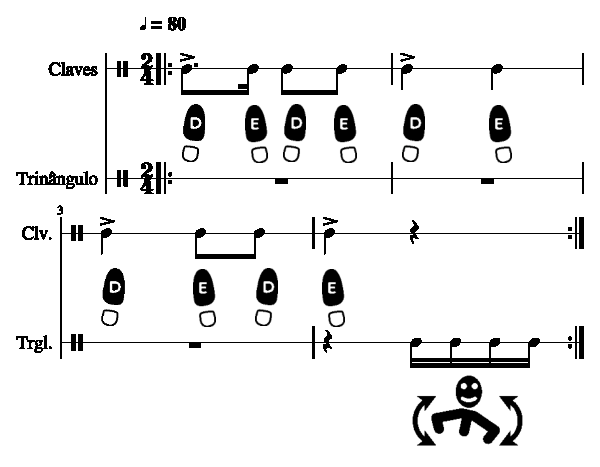
\includegraphics[width=0.9\textwidth]{chapters/cap-musicalidade-tecnica/mickey-mousing-1-1.eps}
    \caption{Treinamento de ``mickey mousing''.}
    \label{fig:mickey-mousing-1-1}
\end{figure}

\begin{example}[Dividindo o corpo em dois instrumentos musicais:]
\label{ex:mickeymousing-2}
Este treinamento é similar ao visto Exemplo \ref{ex:mickeymousing-1};
porem, 
usaremos a frase musical mostrada na Figura \ref{fig:mickey-mousing-2-1}, 
usando os pés seguindo a clave e os ombros seguindo o triangulo.
Os movimentos de ombros no segundo e terceiro compasso
podem ser feitos no \hyperref[def:PlanoFrontal]{\textbf{plano frontal}}.
Já o movimento de ombros no quarto compasso é rápido e livre. 
\end{example}
\begin{figure}[h!]
    \centering
    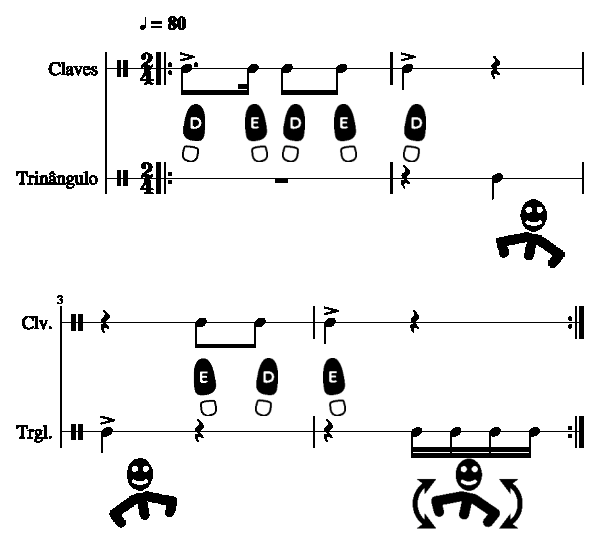
\includegraphics[width=0.99\textwidth]{chapters/cap-musicalidade-tecnica/mickey-mousing-2-1.eps}
    \caption{Treinamento de ``mickey mousing''.}
    \label{fig:mickey-mousing-2-1}
\end{figure}
%\PRLsep{``Mickey mousing'' aplicando tensão e relaxação}

%%%%%%%%%%%%%%%%%%%%%%%%%%%%%%%%%%%%%%%%%%%%%%%%%%%%%%%%%%%%%%%%%%%%%%%%%%%%%%%%
% comprado:
% https://books.google.com.br/books/about/Looking_at_Dances.html?id=Yv6soAEACAAJ&redir_esc=y

%%%%%%%%%%%%%%%%%%%%%%%%%%%%%%%%%%%%%%%%%%%%%%%%%%%%%%%%%%%%%%%%%%%%%%%%%%%%%%%%
% sem preview
% https://books.google.com.br/books?hl=pt-BR&id=fwf0AAAAMAAJ&dq=mickey+mousing&focus=searchwithinvolume&q=mickey+mousing
